\begin{figure}[h!]
\begin{center}
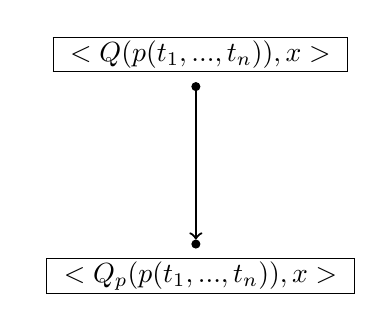
\begin{tikzpicture}[yscale=-1,
place/.style={circle,draw=black, fill=black, inner sep=0pt, 
              minimum size=1mm}]

\node[place] (1st) at (0, 0) [label=above: {
             \begin{tabular}{|c|}
               \hline
              	$<Q(p(t_1,...,t_n)),x>$\\
               \hline
             \end{tabular} }] {};

\node[place] (2nd) at (0, 2) [label=below: {
             \begin{tabular}{|c|}
               \hline
               $<Q_p(p(t_1,...,t_n)),x>$ \\
               \hline
             \end{tabular} }
] {};
        
	\draw[->, thick] (1st) -- (2nd);


\end{tikzpicture}
\end{center}
\caption{Generate new quantifier $Q_p$}
\label{fig:Generating}   
\end{figure}